%!TEX program = xelatex
% 完整编译方法 1 pdflatex -> bibtex -> pdflatex -> pdflatex
% 完整编译方法 2: xelatex -> bibtex -> xelatex -> xelatex
\documentclass[lang=cn,11pt]{elegantpaper}
\usepackage{url}
\usepackage{booktabs}
\usepackage{multirow}
\usepackage{geometry}
\usepackage{longtable}
\usepackage{pdfpages}
\title{写他妈的}

% 不需要版本信息, 直接注释即可
% \version{0.07}
% 不需要时间信息的话, 需要把 \today 删除. 
\date{}


% 如果想修改参考文献样式, 请把这行注释掉
% \usepackage[authoryear]{gbt7714}  % 国标

\begin{document}


\newpage
\Large
\tableofcontents
\thispagestyle{empty}
\newpage
\normalsize
\pagenumbering{arabic}



\section{介绍}
深度学习其实是机器学习的一部分,机器学习经历了从浅层机器学习到深度学习两次浪潮。深度学习模型与浅层机器学习模型之间存在重要区别。浅层机器学习模型不使用分布式表示(distributed representations),而且需要人为提取特征。模型本身只是根据特征进行分类或预测,因此人为提取的特征好坏很大程度上决定了整个系统的好坏。特征提取及特征工程不仅需要专业的领域知识,而且需要花费大量人力物力。深度学习模型是一种表示学习 (representation learning),能够学到数据更高层次的抽象表示,能够自动从数据中提取特征。另外,深度学习的模型能力会随着深度的增加而呈指数增长。
Yann Lecun等人在 1989年提出基于梯度学习的卷积神经网络算法[1],并成功地将其应用在手写数字字符识别,并在当时的技术和硬件条件就能取得低于1\%的错误率。2012年,在计算机视觉“世界杯”之称的ImageNet图像分类竞赛中,Geoffery E.Hinton等人凭借卷积神经网络Alex-Net以超过第二名近12\%的准确率一举夺得该竞赛冠军,霎时间学界业界纷纷惊愕哗然。自此边揭开了卷积神经网络在计算机视觉领域逐渐称霸的序幕,此后每年的ImageNet竞赛的冠军非卷积神经网络莫属。直到2015年,卷积神经网络在ImageNet数据集上的性能(4.94\%)第一次超过了人类预测错误率(5.1\%)。近年来,随着卷积神经网络相关领域研究人员的增多,技术的日新月异,卷积神经网络也变得愈来愈复杂。从最初的5层,16层,到诸如MSRA提出的152层ResNet甚至上千层网络已被广大研究者和工程实践人员司空见惯。
基于CNN在图像识别中已取得的斐然成就,我们将也在各种书籍和课堂的启发下利用现学得的知识搭建一个CNN网络。借助Keras、TensorFlow实现猫狗的图像识别与分类。


\section{CNN网络结构}
在设计网络结构之前,我们必须先要了解我们需要的步骤和所要达到的目的,针对图像识别,一般我们需要以下四步:

\begin{enumerate}
	\item 卷积层初步提取特征.
	\item 池化层提取主要特征.
	\item 全连接层将各部分特征汇总.
	\item 产生分类器,进行预测识别.
\end{enumerate}

\subsection{卷积层}
我们知道假定一个尺寸为$6\times 6$的图像,每一个像素点都储存着图像的信息,那我们可以定义一个卷积核,从图片中提取一定的特征。但机器一开始是无法确定要识别的部分具有哪些特征,所以是通过不同的卷积核相作用得到的输出值,通过比较,可以发现,卷积层输出值越高,越说明匹配程度越高,越能表现给图片的特征。

以要分辨的猫举例,第一层卷积层能学习较小的局部模式(比如猫耳的边缘、瞳孔等),第二层卷积层由第一层特征组成更大的模式(耳朵、眼睛、鼻子),以此类推,形成最终的抽象概念“猫”。

\begin{figure}[hbtp]
	\centering
  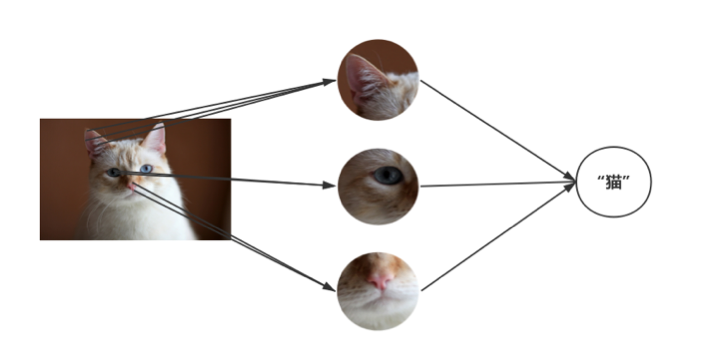
\includegraphics{cat1}
  \caption{视觉世界形成了视觉模块的空间层次结构:比如猫的超局部的边缘组成局部的对象,比如眼镜或耳朵,这些局部对象又组合成高级概念,比如“猫”\label{fig:cat1}}
\end{figure}

卷积的工作原理是在3D特征图上滑动这些$3\times 3$的窗口,在每个可能的位置停止并提取周围特征的3D图块。然后每个3D图块学到的同一个权重矩阵(卷积核)做张量积,转化为1D向量。对这些向量再进行空间重组,转换为3D输出特征图。详细过程见下\figref{fig:conv1},本文将使用Keras的Conv2D层。

\begin{figure}[hbtp]
	\centering
  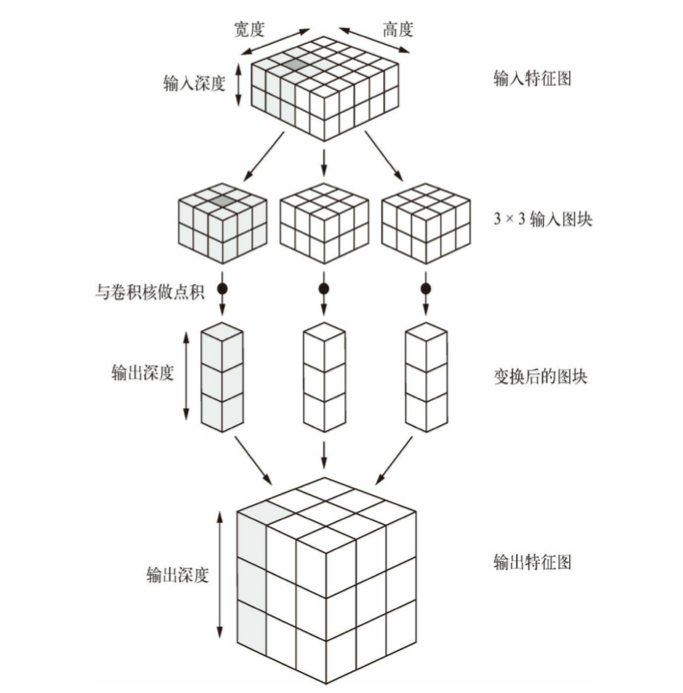
\includegraphics{conv1.png}
  \caption{卷积工作原理.\label{fig:conv1}}
\end{figure}

\subsection{池化层}
池化层的输入就是卷积层输出的原数据与相应的卷积核相乘后的输出矩阵。池化层的目的:
\begin{enumerate}
	\item 为了减少训练参数的数量,降低卷积层输出的特征向量的维度;
	\item 减小过拟合现象,只保留最有用的图片信息,减少噪声的传递;
本文将使用MaxPooling2D从输入特征图中提取窗口,并输入每个通道的最大值。
\end{enumerate}

\subsection{全链接层}

全连接层和卷积层的根本区别在于,全连接层从输入特征空间中学到的是全局模式,而卷积层学到的是局部模式。卷积层和池化层的工作就是提取特征,并减少原始图像带来的参数。然而,为了生成最终的输出,我们需要应用全连接层来生成一个等于我们需要的类的数量的分类器。全连接层的存在大大减少特征位置对分类的影响。
\begin{figure}[hbtp]
\centering
  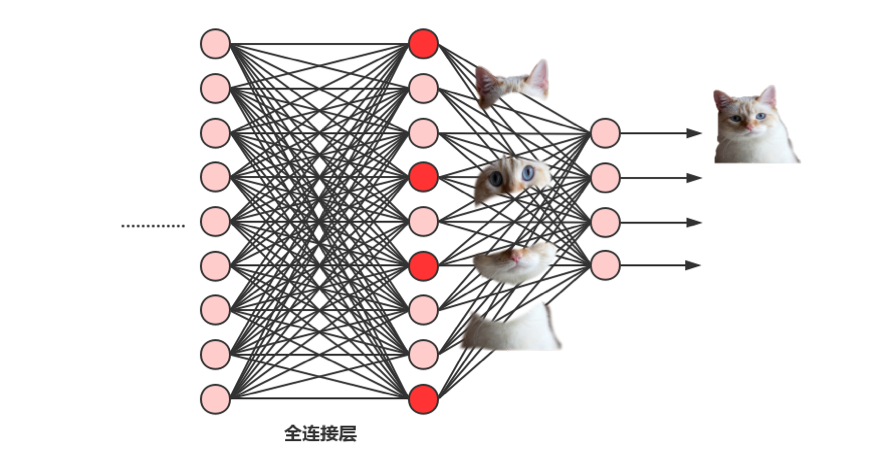
\includegraphics{densecat.png}
  \caption{图中正红色的神经元表示特征被激活了,同一层的其他神经元,要么猫的特征不明显,要么未被发现。当我们把这些特征组合在一起,即为猫. \label{fig:densecat1}}
\end{figure}


\subsection{网络构建}
基于以上的讨论,我们的CNN由Conv2D(使用relu激活)和MaxPooling2D层交替堆叠构成。这里我们使用4个Conv2D+MaxPooling的组合来增大网络容量,也进一步减小特征图的尺寸,使其在连接层Flatten层时尺寸不会太大。由于我们面对的是一个二分类问题,所以网络的最后一层是使用sigmoid激活的单一单元,使用二元交叉熵作为损失函数。


\section{实验过程与结果}

我们在多次尝试配置一台高端机器失败后, 最后选用了一台装备了i7-8700K与单卡GTX1080Ti的机器(keras 2.2.4, tensorflow 1.4.1)上进行了我们简单模型的实验. 因为我们在算力上的短板, 使得我们的模型在全数据上的训练时间过长, 我们不得不在实验的数据量与网络大小上妥协. 但是在这个基础上我们对模型进行了的几次改进, 依旧取得了不错的成果.

\subsection{数据收集与处理}
本文使用Kaggle上的猫狗分类数据集,这个数据集(training的部分)包含25000张猫狗图像(两个类别都有12500张). 我们将其两类分别随机分出了1000张作为训练集, 各500张作为验证集 500张作为测试集数目.

  数据预处理的步骤大致如下:

\begin{enumerate}
	\item 读取图像文件.
	\item 将JPEG文件解码为RGB像素网格($150\times 150$)
	\item 将这些像素网格转换为浮点数张量
	\item 将像素值(0~255范围内)缩放到[0,1]区间
\end{enumerate}

我们调用了Keras的preprocess.image类里的ImageDataGenerator来完成这项工作.

整个数据集被分成了20个batch, 每一个batch有100个样本.

\subsection{第一次试验结果}


\subsection{改进实验细节}

因为我们的算力短板, 我们另寻他路. 希望能够尽量提高在这样的算力能够允许自由实验的前提下达到最好的结果. 我们从第一次试验的结果里可以发现我们的问题主要是算力能够驱动的数据量太小导致了过拟合. 于是我们便引入了预训练模型VGG16与19来进行改进.


\subsubsection{引入预训练VGG16与VGG19}




\subsubsection{数据增强避免过拟合}
由于我们的学习样本并不算海量,可能会出现过拟合的情况,所以我们采用数据增强的方法,利用多种能够生成可信图像的随机变换来增加样本,增强泛化能力。 在Keras中,可以利用ImageDataGenerator实例读取的图像进行多次随机变化,其中的随机变换由多个参数控制,如角度、缩放的范围、平移范围等。

\begin{figure}[hbtp]
\centering
  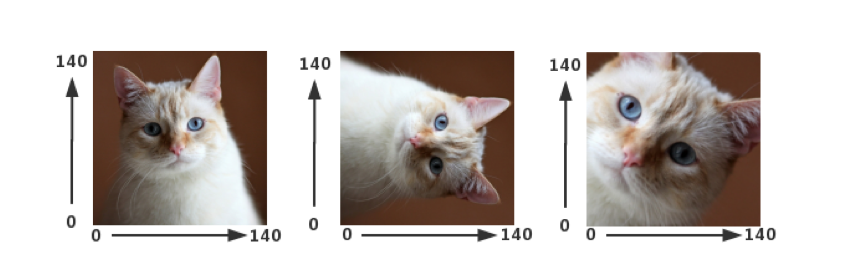
\includegraphics{aug.png}
  \caption{通过随机数据增强生成的猫图像\label{fig:augcat}}
\end{figure}



\section{可视化}

\subsection{可视化中间输出}

\subsection{可视化过滤器}






\newpage
\nocite{*}

% 如果想修改参考文献样式( 非国标 ), 请把下行取消注释, 并换成合适的样式( 比如 unsrt, plain 样式 ). 
\bibliographystyle{unsrt}
\bibliography{wpref}

\end{document}
